\documentclass[12pt, letterpaper]{article}
\usepackage[utf8]{inputenc}
\usepackage{indentfirst}
\usepackage{graphicx}
\usepackage{setspace}
\usepackage[numbers]{natbib}
\usepackage [autostyle, english = american]{csquotes}
\MakeOuterQuote{"}
\usepackage{layout}
\usepackage[title]{appendix}
\usepackage[justification=centering]{caption}
\usepackage{titlesec}
\usepackage[percent]{overpic}
\usepackage{amsmath}
\usepackage{systeme}
\usepackage{blkarray, bigstrut}
\usepackage{tikz}
\usetikzlibrary{tikzmark}
\usepackage[utf8]{inputenc}
\usepackage{relsize}
\usepackage[nameinlink, capitalize, noabbrev]{cleveref}
\usepackage{tabu}

\setlength\parskip{\baselineskip}

%prevent hyphenation of words
%\emergencystretch=\maxdimen
\hyphenpenalty=10000
\hbadness=10000

\begin{document}

\setcounter{secnumdepth}{-1}
\titlespacing*{\section}{0pt}{1.5\baselineskip}{.25\baselineskip}
\binoppenalty=\maxdimen
\relpenalty=\maxdimen

\setlength{\abovedisplayskip}{-\baselineskip}
\setlength{\belowdisplayskip}{0\baselineskip}
\setlength{\abovedisplayshortskip}{0\baselineskip}


%Cover page: 5pts
%Course, subject, name, date
\title{MA348 Numerical Analysis, Differential Equations}
\author{David Jefts}
\date{April 27\textsuperscript{th}, 2019}
\begin{titlepage}
	\centering
	\maketitle
	\centering
	\hfill
	\vfill
	\thispagestyle{empty}
\end{titlepage}

\setlength{\voffset}{-0.5in}
\setlength{\headsep}{10pt}

%Introduction: 5pts
%Describe the problem and state objectives
\section{\label{sec:intro}Introduction}
	%Runge-Kutta Methods
	The purpose of this lab is to develop a method of numerical analysis and then generate software to use and apply that method. This lab is based on the First-Order Runge-Kutta (RK) Iterative Methods to solve Ordinary Differential Equations (ODEs) of the form $\frac{dy}{dx}=f(x,y)$
	 
	 The Runge-Kutta methods are iterative methods that are all based off of the formula,
	 
	 \begin{equation}y_{i+1}=y_i + \phi h\end{equation}
	 
	 where $y_{i+1}$ is the new value being extrapolated, $y_i$ is the previous value, $\phi$ is a slope estimate, and $h$ is the step size. The iterative estimating based on the previous estimate requires that an initial $y$ value be given for each of the methods.
	 
	 This lab is based off of the example equations below and will be comparing the effectiveness of Euler's Method and Heun's Method in terms of speed, ease of use, and accuracy for both types of equations. 
	 
	  \begin{equation}\frac{dy}{dx}=-2x^3+12x^2-20x+8.5\end{equation}
	  
	  \begin{equation}\frac{dy}{dx}=4e^{0.8x}-0.5y\end{equation}

%Theory-Analysis: 5pts
%State assumptions and develop equations
\section{\label{sec:theory}Theory-Analysis}
	All of the following methods are different ways to solve a linear Ordinary Differential Equation (ODE) and are based around using the slope and the previously estimated function value to iteratively estimate the next $y$ value of the function. All methods follow the general formula $y_{i+1}=y_i + \phi h$ where $\phi$ is the slope function and is calculate differently for each of the methods.
	
	Euler's method substitutes $\phi$ with only the original differential equation: $y_{i+1}=y_i + f(x_i, y_i) h$ where $f(x_i, y_i)=\frac{dy}{dx}$. The method is iterated with a step size of $h$ starting with the initial $x$ value ($x=0.0$), the final $x$ value ($x=4.0$), and an initial $y$ value ($y=1.0$).
	
	Heun's Method is an expansion upon Euler's Method that adds a \textit{correction function} that is used to help bring the estimate differential value closer to the actual value. It creates an initial estimate using the same function as Euler's method, but then uses that initial estimate to create a new estimate than averages those two estimates together to get the slope, $\phi$.
	
	\begin{equation}y_{old}=y_{previous} + f(x_i, y_i)h\end{equation}
	\begin{equation}y_{new} = y_{previous} + f(x_i+h, y_{old})h\end{equation}
	
	\begin{equation*}\phi=\frac{y_{old}+y_{new}}{2}\end{equation*}
	
	So the final iterative equation used for the Heun Method is $y_{i+1}=y_i+\frac{y_{old}+y_{new}}{2}h$
	
	There were no assumptions in this lab, and the analytical solutions for Equations (1) and (2) are:
	
		\begin{equation*}-0.5x^4+4x^3-10x^2+8.5x+1\end{equation*}
		\begin{equation*}\frac{4}{1.3}\left(e^{0.8x}-e^{-0.5x}\right)+2e^{-0.5x}\end{equation*}

	 
%Numerical Solution: 20pts
%Describe the numerical methods used to solve the problem
\section{\label{solution}Numerical Solution}
	All of the methods were coded in Python, with this report created in \LaTeX{}.
	
	Euler's Method, also known as the Euler-Cauchy Method or the Point-Slope Method, is a basic one-step method used to estimate the solution to Ordinary Differential Equations (ODEs). It uses the differential equation directly to estimate the slope in the form of the first derivative starting at $x_i$, the initial $x$ value. This original slope is used as an approximation of the slope of the entire step-sized interval. With Euler's Method, each new $y$ value is extrapolated linearly over each step size of $h$ using the following formula:
	
	\begin{equation}y_{i+1}=y_i+f(x_i, y_i)h\end{equation}
	
	Since this equation is based on a Taylor Series expansion one could include additional terms to increase the order of the estimation function, however each additional term requires the calculation of the next derivative of the ODE. For example, the next Taylor Series term for the above equation is $\frac{f'(x_i,y_i)}{2!}h^2$ while the term after that would be $\frac{f''(x_i,y_i)}{3!}h^3$. In the Python Software developed for this lab, Equation (6) is placed inside of a loop that iterates over the $x$ values, with each iteration adding the step size, $h$, to $x$ and updating the $y$ value. The absolute error is determined by $\left|f(x)-y_i\right|$ where $f(x)$ is the solved differential equation. The table of all of these values can be found in the Results and Discussion section. 
	
	Heun's Method improves upon Euler's Method by improving the accuracy of the slope determination. It does this by finding the slope at each end of the interval and averaging them together, then using that as the new slope ($\phi$) value. In Euler's Method, the $y_i'=f(x_i,y_i)$, is used to extrapolate linearly to $y_{i+1}^0=y_i+f(x_i, y_i)h$. However, Heun's Method adds another step, using $y_{i+1}^0$ as a predictor function to estimate a new slope at the end of the interval, $y_{i+1}'=f(x_{i+1},y_{i+1}^0)$. These two slope functions can then be averaged to create a new $\phi$ equation, $\phi=\frac{y_i'+y_{i+1}'}{2}=\frac{f(x_i, y_i)+f(x_{i+1},y_{i+1}^0)}{2}$. The final corrector equation is then:
	
	\begin{equation}y_{i+1}=y_i+\frac{f(x_i, y_i)+f(x_{i+1},y_{i+1}^0)}{2}h\end{equation}
	
	These two steps, determining the predictor equation and the corrector equation, are then iterated $x_i$ up through $x_f$ by the step size of $h$, for a total of $\frac{x_i-x_f}{h}$ iterations. The error is determined with the same formula as Euler's Method.
	 

%Results and Discussion: 45pts
%Tabulate and plot the results, compare results, and discuss the accuracy of results
\section{\label{sec:results}Results and Discussion}
    	The following table is based on a step size of 0.5 on the interval of $[0,4]$:
	
	\begin{table}[h]
	\centering
	\begin{tabular}{c|cc|cc}
	x & Euler's Method & Euler's Error & Heun's Method & Heun's Error \\ \hline
	0.00 & 1.00000 & 0.00000 & 1.00000 & 0.00000 \\
	0.50 & 5.25000 & 2.03125 & 3.43750 & 0.21875 \\
	1.00 & 5.87500 & 2.87500 & 3.37500 & 0.37500 \\
	1.50 & 5.12500 & 2.90625 & 2.68750 & 0.46875 \\
	2.00 & 4.50000 & 2.50000 & 2.50000 & 0.50000 \\
	2.50 & 4.75000 & 2.03125 & 3.18750 & 0.46875 \\
	3.00 & 5.87500 & 1.87500 & 4.37500 & 0.37500 \\
	3.50 & 7.12500 & 2.40625 & 4.93750 & 0.21875 \\
	4.00 & 7.00000 & 4.00000 & 3.00000 & 0.00000
	\end{tabular}
	\end{table}
	
	\newpage
	These methods can both be improved by reducing the step size:
	
	\begin{table}[h]
	\centering
	\begin{tabular}{c|cc|cc|c}
	x & Euler's Method & Euler's Error & Heun's Method & Heun's Error & Actual \\ \hline
	0.00 & 1.00000 & 0.00000 & 1.00000 & 0.00000 & 1.00000 \\
	0.25 & 3.12500 & 0.56445 & 2.58984 & 0.02930 & 2.56055 \\
	0.50 & 4.17969 & 0.96094 & 3.27344 & 0.05469 & 3.21875 \\
	0.75 & 4.49219 & 1.21289 & 3.35547 & 0.07617 & 3.27930 \\
	1.00 & 4.34375 & 1.34375 & 3.09375 & 0.09375 & 3.00000 \\
	1.25 & 3.96875 & 1.37695 & 2.69922 & 0.10742 & 2.59180 \\
	1.50 & 3.55469 & 1.33594 & 2.33594 & 0.11719 & 2.21875 \\
	1.75 & 3.24219 & 1.24414 & 2.12109 & 0.12305 & 1.99805 \\
	2.00 & 3.12500 & 1.12500 & 2.12500 & 0.12500 & 2.00000 \\
	2.25 & 3.25000 & 1.00195 & 2.37109 & 0.12305 & 2.24805 \\
	2.50 & 3.61719 & 0.89844 & 2.83594 & 0.11719 & 2.71875 \\
	2.75 & 4.17969 & 0.83789 & 3.44922 & 0.10742 & 3.34180 \\
	3.00 & 4.84375 & 0.84375 & 4.09375 & 0.09375 & 4.00000 \\
	3.25 & 5.46875 & 0.93945 & 4.60547 & 0.07617 & 4.52930 \\
	3.50 & 5.86719 & 1.14844 & 4.77344 & 0.05469 & 4.71875 \\
	3.75 & 5.80469 & 1.49414 & 4.33984 & 0.02930 & 4.31055 \\
	4.00 & 5.00000 & 2.00000 & 3.00000 & 0.00000 & 3.00000
	\end{tabular}
	\end{table}


%Conclusions: 20pts
%Comment on the efficiency of the solvers
\section{\label{conclusion}Conclusions}
	Both Euler's Method and Heun's Method are very effective at estimating the solution values for Ordinary Differential Equations but Heun's Method routinely resulted in more accurate values. To contrast that, Euler's Method was considerably easier to implement and requires less memory to operate, both physical storage space and short-term space. Euler's Method is also very easy to apply even though the error increases and propagates at a much faster rate. In conclusion, Heun's method should generally be preferred since it does not take much more effort to apply than Euler's Method. 

\pagebreak
%Appendices
%Include listings of the source codes, include printed copies of the output files
\appendix
	\section{Appendix A}
            	\begin{figure}[h]
            		\centering
            		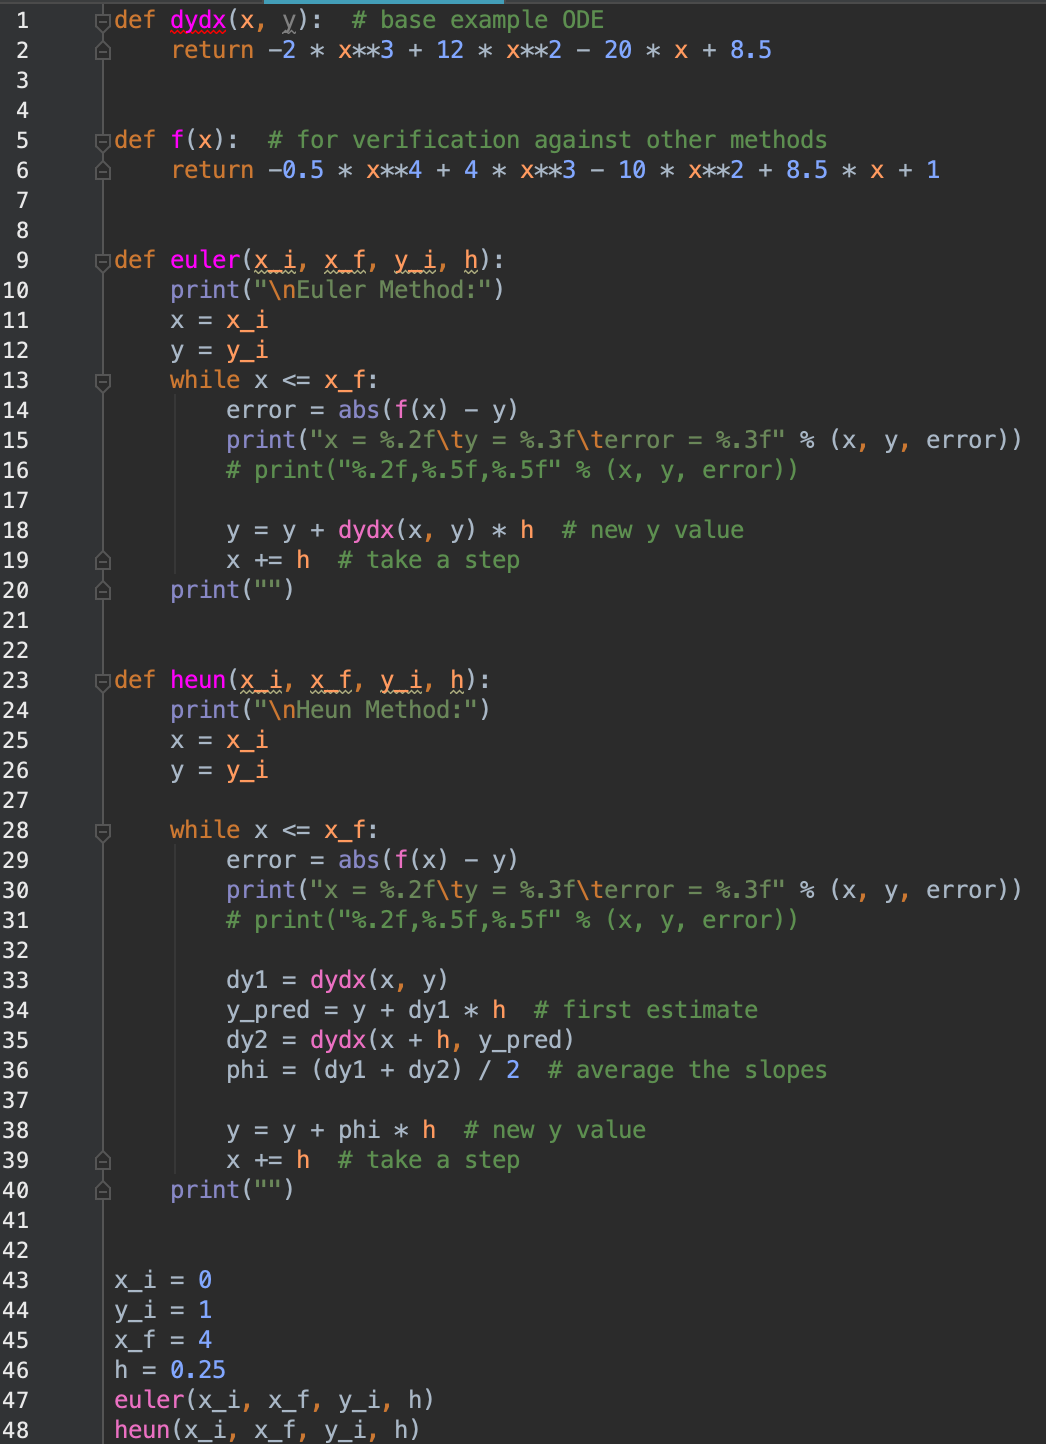
\includegraphics[width=0.78899\linewidth]{PythonCode.png}
            	\end{figure}
		
		
		


\end{document}
